% Options for packages loaded elsewhere
\PassOptionsToPackage{unicode}{hyperref}
\PassOptionsToPackage{hyphens}{url}
\PassOptionsToPackage{dvipsnames,svgnames,x11names}{xcolor}
%
\documentclass[
  letterpaper,
  DIV=11,
  numbers=noendperiod]{scrartcl}

\usepackage{amsmath,amssymb}
\usepackage{lmodern}
\usepackage{iftex}
\ifPDFTeX
  \usepackage[T1]{fontenc}
  \usepackage[utf8]{inputenc}
  \usepackage{textcomp} % provide euro and other symbols
\else % if luatex or xetex
  \usepackage{unicode-math}
  \defaultfontfeatures{Scale=MatchLowercase}
  \defaultfontfeatures[\rmfamily]{Ligatures=TeX,Scale=1}
\fi
% Use upquote if available, for straight quotes in verbatim environments
\IfFileExists{upquote.sty}{\usepackage{upquote}}{}
\IfFileExists{microtype.sty}{% use microtype if available
  \usepackage[]{microtype}
  \UseMicrotypeSet[protrusion]{basicmath} % disable protrusion for tt fonts
}{}
\makeatletter
\@ifundefined{KOMAClassName}{% if non-KOMA class
  \IfFileExists{parskip.sty}{%
    \usepackage{parskip}
  }{% else
    \setlength{\parindent}{0pt}
    \setlength{\parskip}{6pt plus 2pt minus 1pt}}
}{% if KOMA class
  \KOMAoptions{parskip=half}}
\makeatother
\usepackage{xcolor}
\setlength{\emergencystretch}{3em} % prevent overfull lines
\setcounter{secnumdepth}{-\maxdimen} % remove section numbering
% Make \paragraph and \subparagraph free-standing
\ifx\paragraph\undefined\else
  \let\oldparagraph\paragraph
  \renewcommand{\paragraph}[1]{\oldparagraph{#1}\mbox{}}
\fi
\ifx\subparagraph\undefined\else
  \let\oldsubparagraph\subparagraph
  \renewcommand{\subparagraph}[1]{\oldsubparagraph{#1}\mbox{}}
\fi


\providecommand{\tightlist}{%
  \setlength{\itemsep}{0pt}\setlength{\parskip}{0pt}}\usepackage{longtable,booktabs,array}
\usepackage{calc} % for calculating minipage widths
% Correct order of tables after \paragraph or \subparagraph
\usepackage{etoolbox}
\makeatletter
\patchcmd\longtable{\par}{\if@noskipsec\mbox{}\fi\par}{}{}
\makeatother
% Allow footnotes in longtable head/foot
\IfFileExists{footnotehyper.sty}{\usepackage{footnotehyper}}{\usepackage{footnote}}
\makesavenoteenv{longtable}
\usepackage{graphicx}
\makeatletter
\def\maxwidth{\ifdim\Gin@nat@width>\linewidth\linewidth\else\Gin@nat@width\fi}
\def\maxheight{\ifdim\Gin@nat@height>\textheight\textheight\else\Gin@nat@height\fi}
\makeatother
% Scale images if necessary, so that they will not overflow the page
% margins by default, and it is still possible to overwrite the defaults
% using explicit options in \includegraphics[width, height, ...]{}
\setkeys{Gin}{width=\maxwidth,height=\maxheight,keepaspectratio}
% Set default figure placement to htbp
\makeatletter
\def\fps@figure{htbp}
\makeatother

\KOMAoption{captions}{tableheading}
\makeatletter
\makeatother
\makeatletter
\makeatother
\makeatletter
\@ifpackageloaded{caption}{}{\usepackage{caption}}
\AtBeginDocument{%
\ifdefined\contentsname
  \renewcommand*\contentsname{Table of contents}
\else
  \newcommand\contentsname{Table of contents}
\fi
\ifdefined\listfigurename
  \renewcommand*\listfigurename{List of Figures}
\else
  \newcommand\listfigurename{List of Figures}
\fi
\ifdefined\listtablename
  \renewcommand*\listtablename{List of Tables}
\else
  \newcommand\listtablename{List of Tables}
\fi
\ifdefined\figurename
  \renewcommand*\figurename{Figure}
\else
  \newcommand\figurename{Figure}
\fi
\ifdefined\tablename
  \renewcommand*\tablename{Table}
\else
  \newcommand\tablename{Table}
\fi
}
\@ifpackageloaded{float}{}{\usepackage{float}}
\floatstyle{ruled}
\@ifundefined{c@chapter}{\newfloat{codelisting}{h}{lop}}{\newfloat{codelisting}{h}{lop}[chapter]}
\floatname{codelisting}{Listing}
\newcommand*\listoflistings{\listof{codelisting}{List of Listings}}
\makeatother
\makeatletter
\@ifpackageloaded{caption}{}{\usepackage{caption}}
\@ifpackageloaded{subcaption}{}{\usepackage{subcaption}}
\makeatother
\makeatletter
\@ifpackageloaded{tcolorbox}{}{\usepackage[many]{tcolorbox}}
\makeatother
\makeatletter
\@ifundefined{shadecolor}{\definecolor{shadecolor}{rgb}{.97, .97, .97}}
\makeatother
\makeatletter
\makeatother
\ifLuaTeX
  \usepackage{selnolig}  % disable illegal ligatures
\fi
\IfFileExists{bookmark.sty}{\usepackage{bookmark}}{\usepackage{hyperref}}
\IfFileExists{xurl.sty}{\usepackage{xurl}}{} % add URL line breaks if available
\urlstyle{same} % disable monospaced font for URLs
\hypersetup{
  pdftitle={Brighton and Hove Secondary School Admissions - Factsheet},
  pdfauthor={Professor Adam Dennett FRGS FAcSS, Professor of Urban Analytics, Bartlett Centre for Advanced Spatial Analysis, University College London - a.dennett@ucl.ac.uk - @adam\_dennett},
  colorlinks=true,
  linkcolor={blue},
  filecolor={Maroon},
  citecolor={Blue},
  urlcolor={Blue},
  pdfcreator={LaTeX via pandoc}}

\title{Brighton and Hove Secondary School Admissions - Factsheet}
\author{Professor Adam Dennett FRGS FAcSS, Professor of Urban Analytics,
Bartlett Centre for Advanced Spatial Analysis, University College London
- a.dennett@ucl.ac.uk - @adam\_dennett}
\date{}

\begin{document}
\maketitle
\ifdefined\Shaded\renewenvironment{Shaded}{\begin{tcolorbox}[sharp corners, enhanced, borderline west={3pt}{0pt}{shadecolor}, interior hidden, frame hidden, boxrule=0pt, breakable]}{\end{tcolorbox}}\fi

\hypertarget{fact-1---disadvantaged-attainment}{%
\subsection{Fact 1 - Disadvantaged
Attainment}\label{fact-1---disadvantaged-attainment}}

In 2024, all students in Brighton and Hove - both disadvantaged and
non-disadvantaged - achieved \textbf{\emph{ABOVE}} the national (median)
average when compared to other Local Authorities (both Upper and Lower
Tier) in England. There is an attainment gap between disadvantaged and
non-disadvantaged pupils in every Local Authority in England. Brighton's
is an artefact of non-disadvantaged students doing far better than
average.

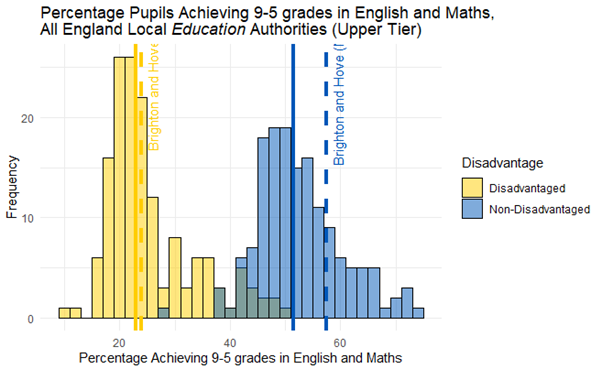
\includegraphics{images/attainmentgap_95.png}

\url{https://adamdennett.github.io/BH_Schools_2/stain_removal.html\#disadvantaged-vs-non-disadvantaged-pupils}

\hypertarget{fact-2---school-demand}{%
\subsection{Fact 2 - School Demand}\label{fact-2---school-demand}}

Demand for schools varies significantly across the city. At the lower
end, in the last 11-years, Longhill has received fewer
\textbf{\emph{total applications}} (1st, 2nd and 3rd choice combined)
than its Published Admission Number (PAN) of 270. For comparison,
another single catchment school - Patcham High, has generally received
around twice as many total applications than PAN.

Over the last 11 years (since 2013), Longhill's total offers have
trended down every year, and it has never achieved anywhere near 270
offers. It's peak was in 2014 when it made 209 offers. Last year it made
94 offers.

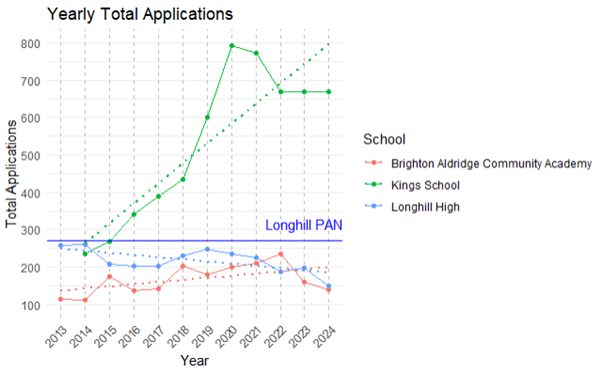
\includegraphics{images/yearly_apps_sml.png}

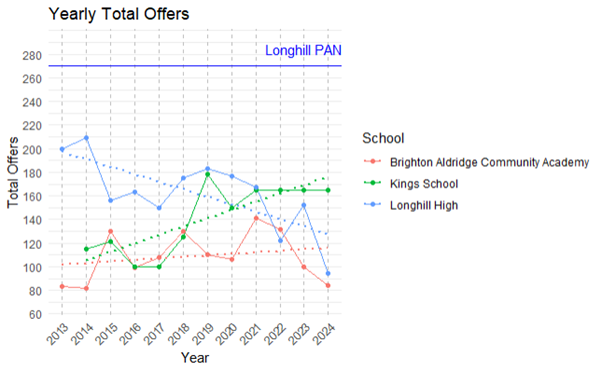
\includegraphics{images/yearly_offers_sml.png}

\url{https://adamdennett.github.io/BH_Schools_2/schools_wk2.html\#school-application-and-offer-history-across-brighton}

\hypertarget{fact-3---geodemographic-reality}{%
\subsection{Fact 3 - Geodemographic
Reality}\label{fact-3---geodemographic-reality}}

School children in Brighton and Hove are not distributed evenly across
the city and not all school locations correspond to where pupils live.
Both Longhill and, to a lesser extent, BACA are located away from where
students current live and are likely to live in the future. Any desire
to ``Maintain the geographic spread of secondary schools in the city''
makes no sense if that spread bears no relation to where children live.

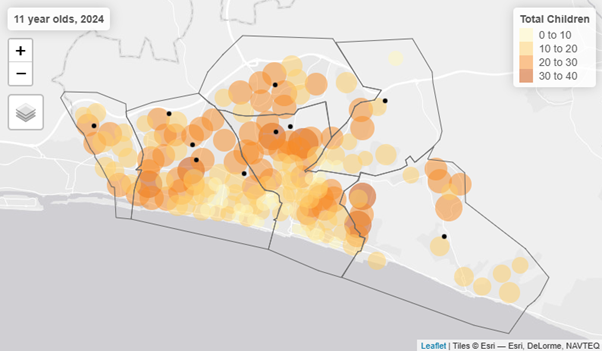
\includegraphics{images/map_11_year_olds_2024.png}

\url{https://adamdennett.github.io/BH_Schools_2/schools_wk3.html\#a-model-of-brightopia}

\hypertarget{fact-4---demographic-decline-and-pan-reductions}{%
\subsection{Fact 4 - Demographic Decline and PAN
reductions}\label{fact-4---demographic-decline-and-pan-reductions}}

Brighton and Hove's student population will decline over the next
decade. It is unlikely that this decline will be even across the city.
Current proposed PAN reductions for schools in the city are not
equitable as they ignore likely future demand, even as total populations
of students decline.

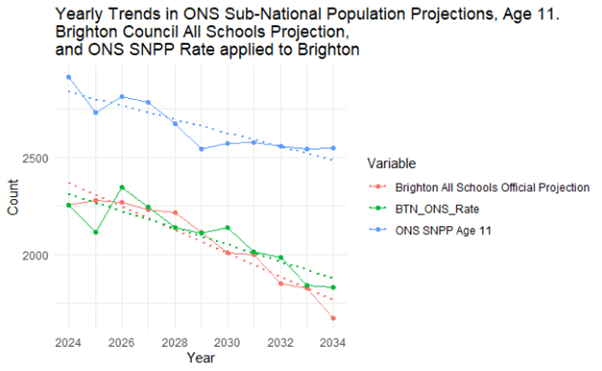
\includegraphics{images/pop_proj.png}

\url{https://adamdennett.github.io/BH_Schools_2/schools_wk2.html\#comparing-brighton-pan-projections-with-ons-sub-national-population-projections}

\hypertarget{fact-5---school-size}{%
\subsection{Fact 5 - School Size}\label{fact-5---school-size}}

11-16 state-run schools exist and thrive in England and Wales with PANs
smaller than 180. One already exists in Brighton. A school with a PAN of
150 would still exist near the centre of the national school size
distribution for 11-16 secondary schools.

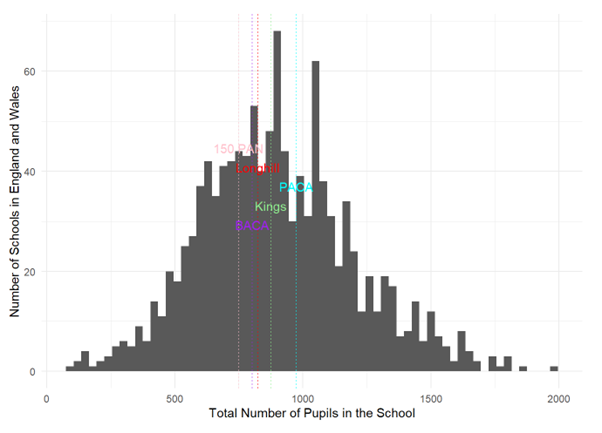
\includegraphics{images/school_size_hist.png}

\url{https://adamdennett.github.io/BH_Schools_2/schools_wk2.html\#pan-2026-scenario-3---the-kings-scenario}

\hypertarget{fact-6---travel-distance-to-school}{%
\subsection{Fact 6 - Travel distance to
school}\label{fact-6---travel-distance-to-school}}

Most pupils in towns and cities the UK and Europe don't travel very far
to secondary school (\textless3km). Some children in Brighton and Hove,
under current catchment arrangements (particularly those who live in
Whitehawk) do have to travel far (\textgreater5km) and have no option to
walk to school. Most children from Whitehawk currently have to attend
Longhill, which is a bus journey away.

Under Option B, significant numbers of children
(\href{https://adamdennett.github.io/BH_Schools_2/schools_wk3.html\#option-b-and-the-inevitable-mass-transfer-of-children-from-central-brighton-to-the-east}{estimates
of up to 365 a day}) from central Brighton would be forced to to travel
4-5 miles (6-8km) to attend school at Longhill - a distance more common
in sparse rural areas. This would be an unusually long distance and a
journey which currently takes 1 to 1.5hrs on public transport, each way;
so 2-3hrs a day of travelling if public transport were used.

In a world recognising the benefits of the `15-minute city' -
\url{https://www.moreno-web.net/new-book-the-15-minute-city-a-solution-to-saving-our-time-and-our-planet/}
- forcing more long-distance travel would be a regressive policy. The
Brighton and Hove School Model of Travel Survey found, in 2024, that
26.2\% of journeys to and from secondary school were made by car.
\url{https://www.brighton-hove.gov.uk/travel-and-road-safety/travel-transport-and-road-safety/school-mode-travel-survey-2024-guidance-letter}

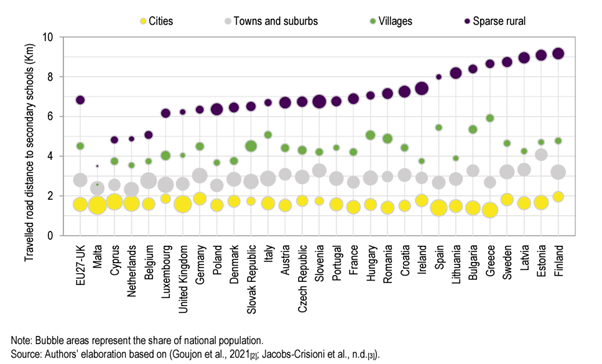
\includegraphics{images/distance_europe.png}

Source:
\url{https://www.oecd.org/en/publications/2021/06/access-and-cost-of-education-and-health-services_4889b7a5/full-report/component-7.html\#figure-d1e11132}

\hypertarget{fact-7---statistical-smoothing-is-not-improvement}{%
\subsection{Fact 7 - Statistical Smoothing is not
`improvement'}\label{fact-7---statistical-smoothing-is-not-improvement}}

Redrawing boundaries and enlarging catchments may give the illusion of
`improvement' in the distribution of things like Free School Meals, when
really everything is just moving closer to the city average.

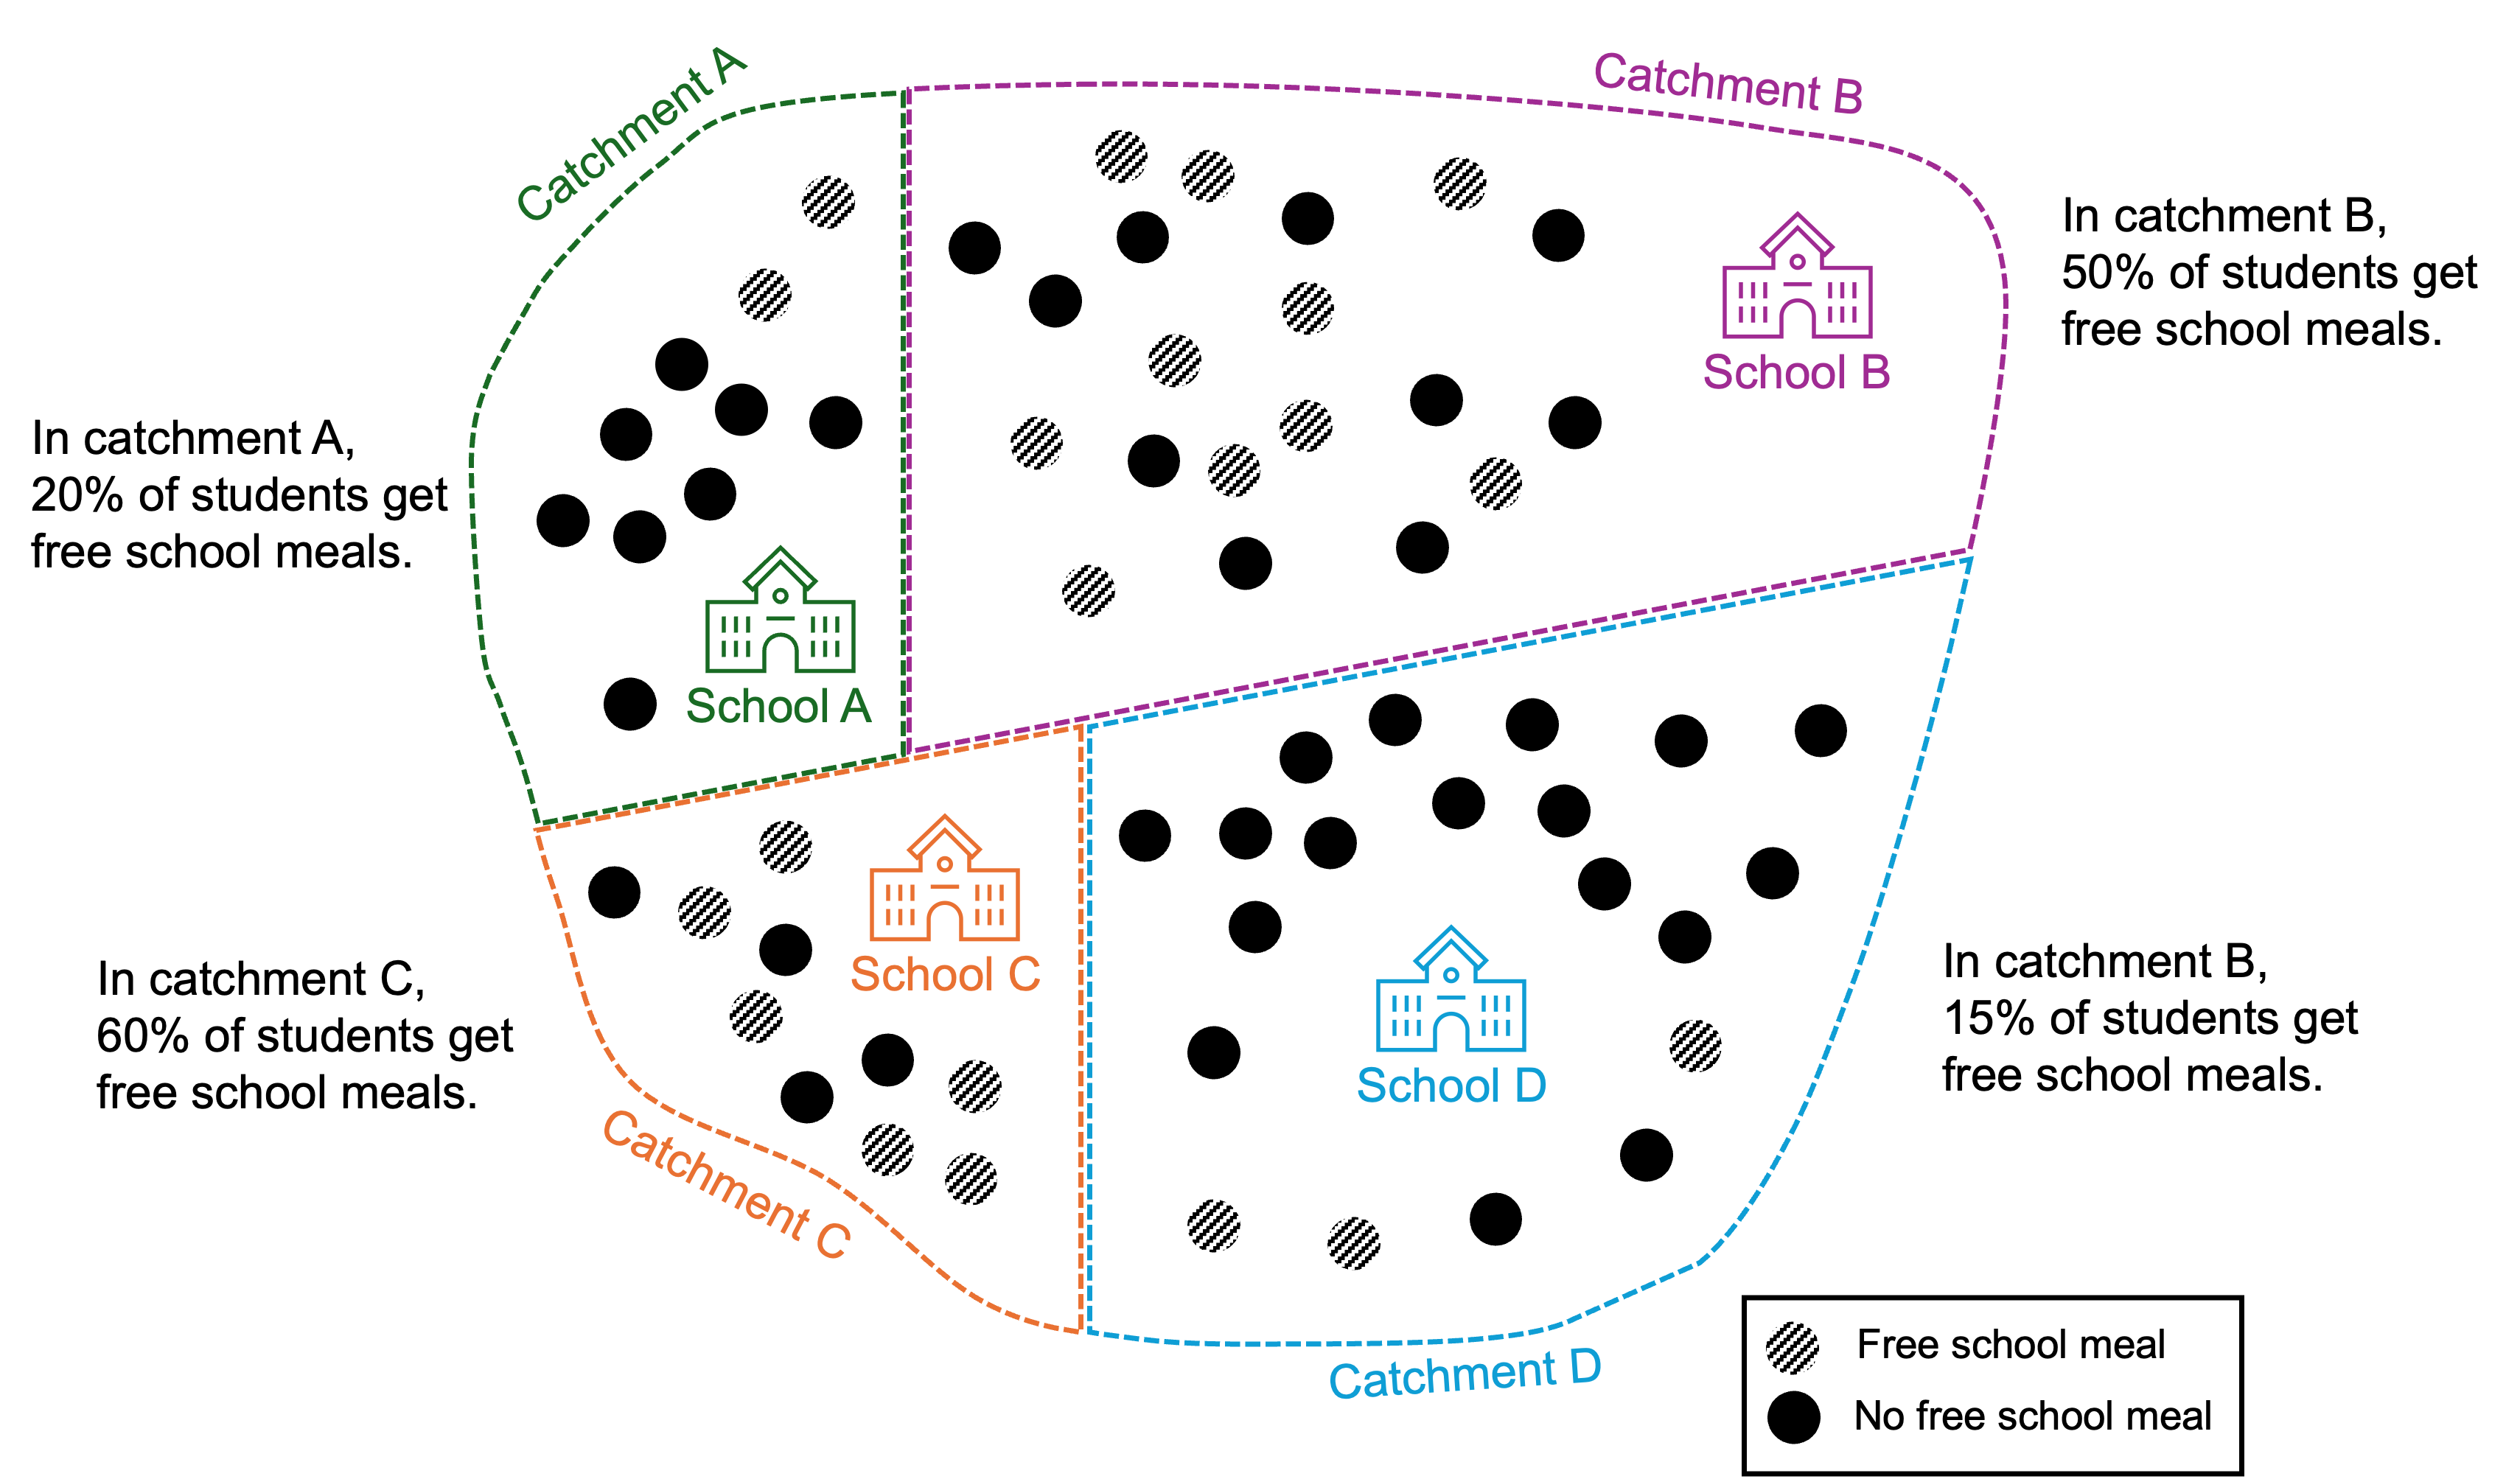
\includegraphics[width=0.5\textwidth,height=\textheight]{images/stat_smoothing_1.png}

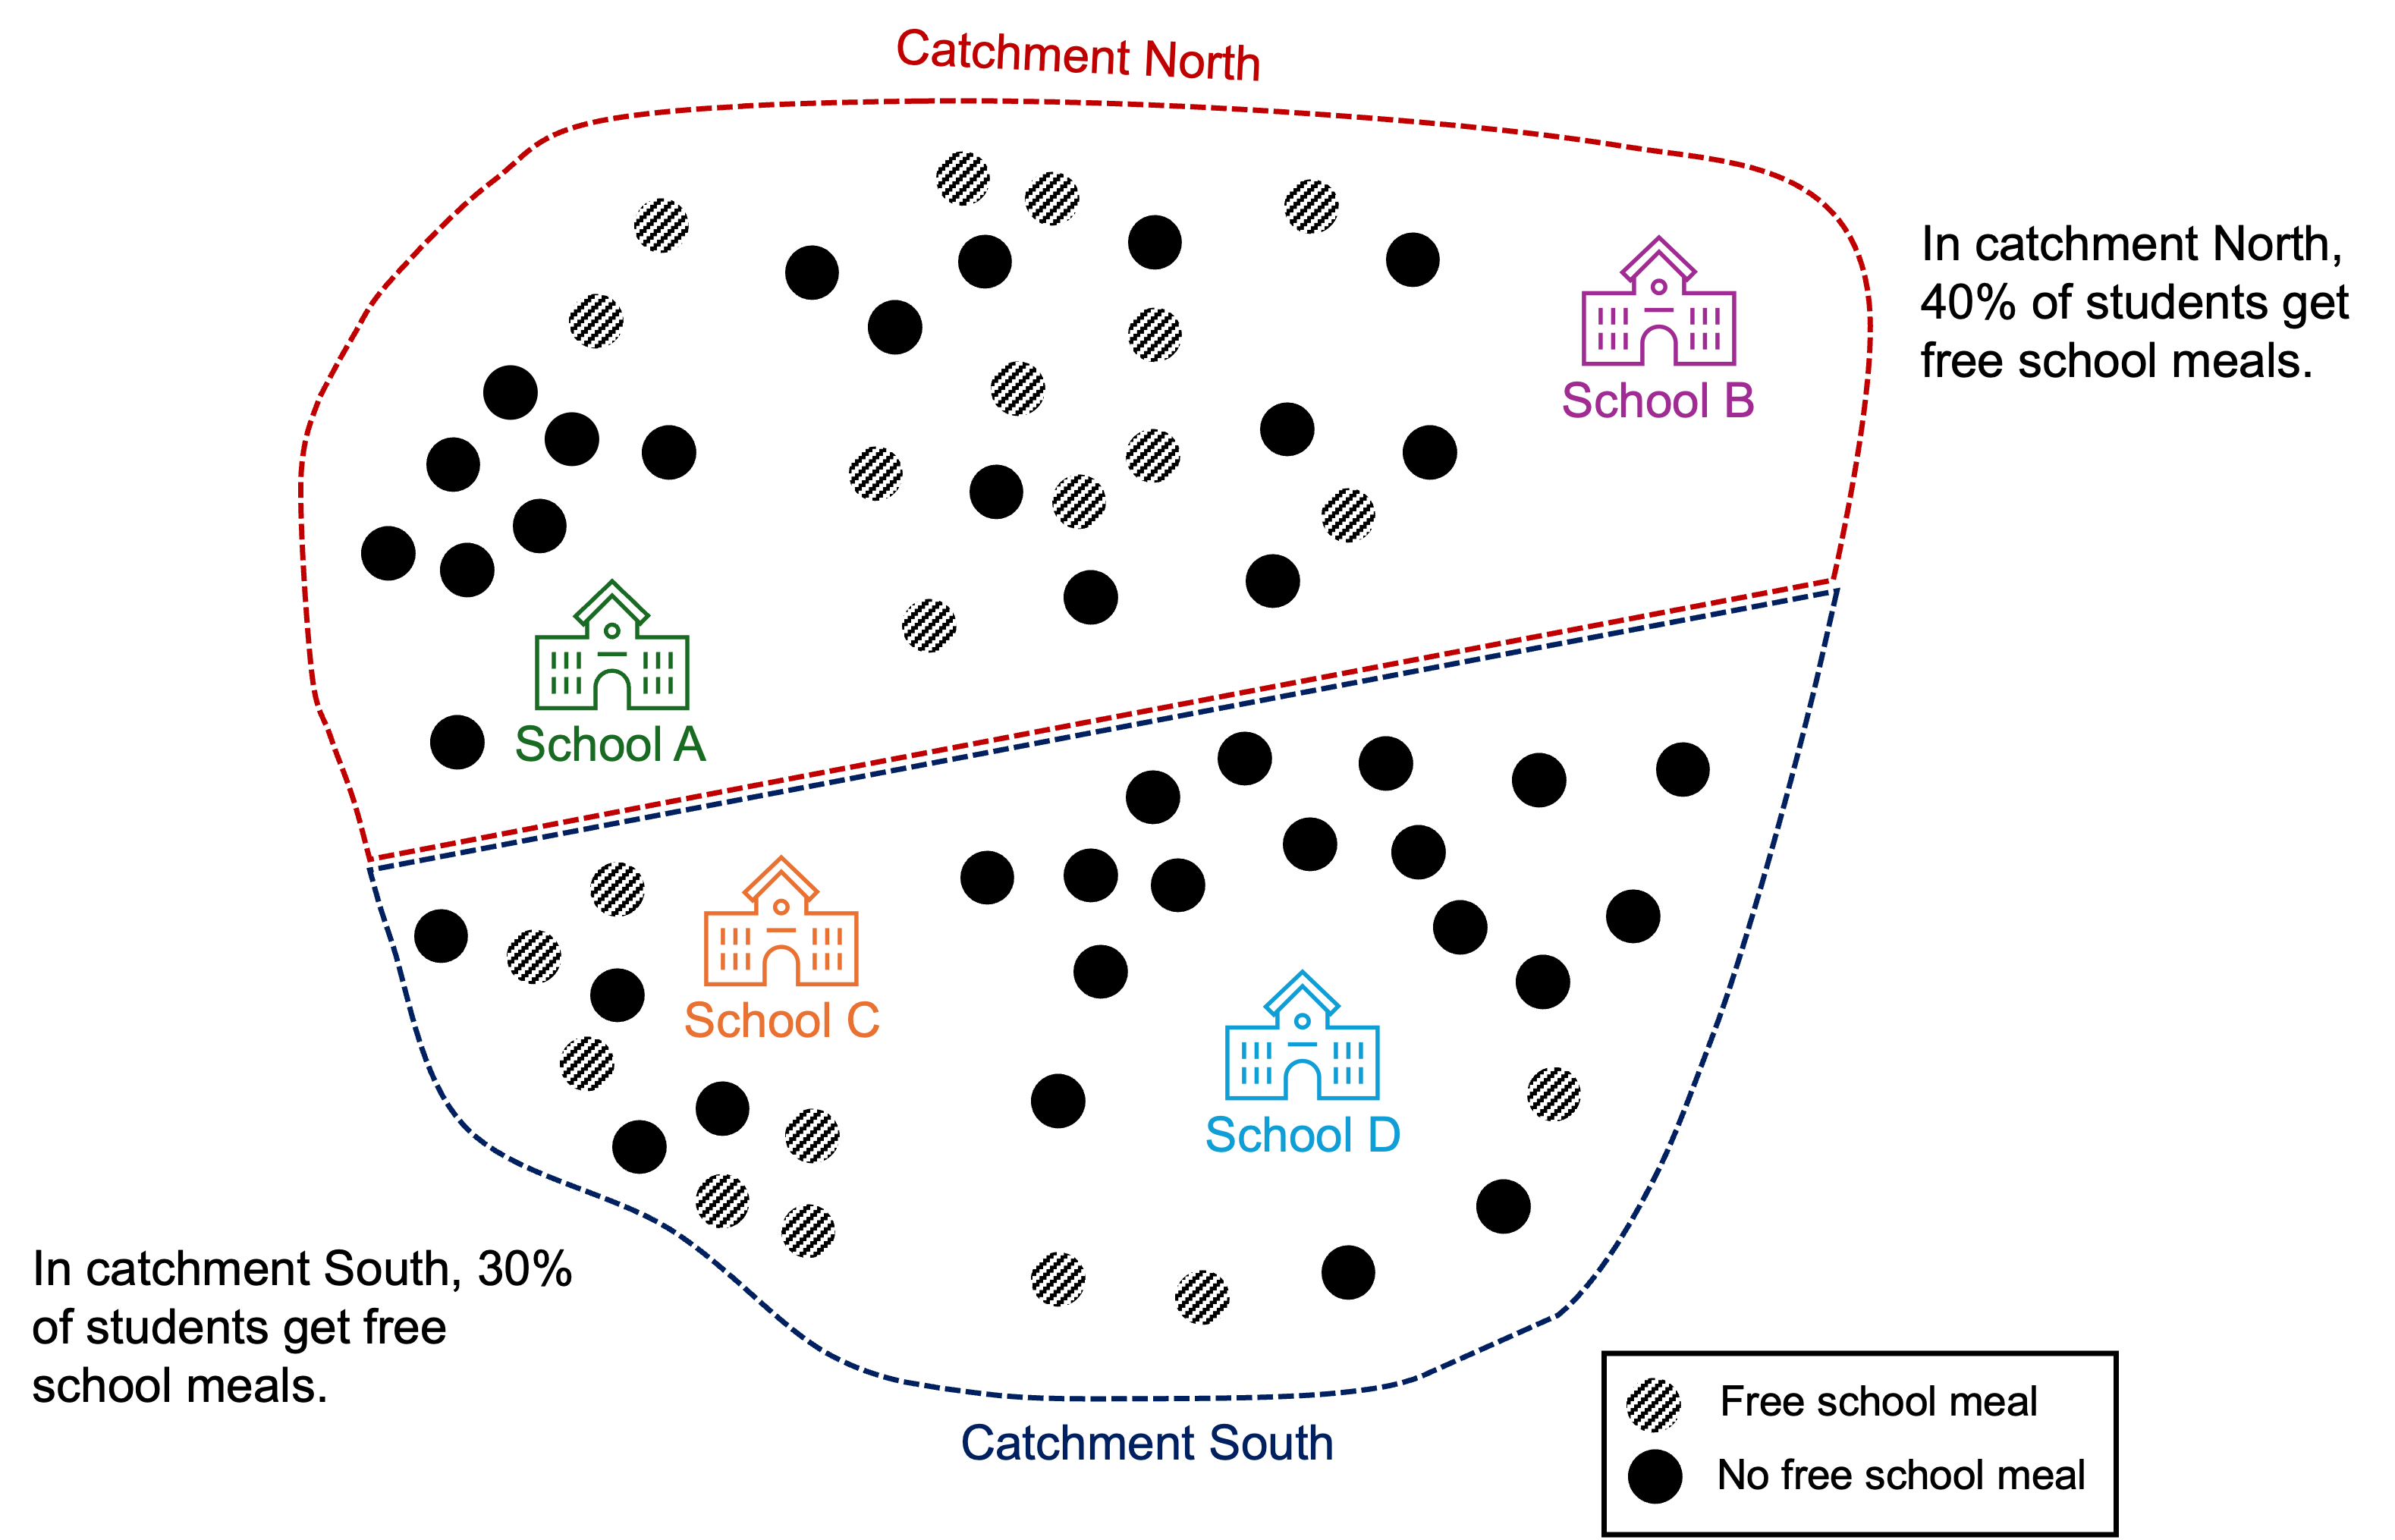
\includegraphics[width=0.5\textwidth,height=\textheight]{images/stat_smoothing_2.png}

\url{https://adamdennett.github.io/BH_Schools_2/schools_wk3.html\#statistical-smoothing}

\hypertarget{factsheet---additional-info}{%
\section{Factsheet - Additional
Info}\label{factsheet---additional-info}}

\hypertarget{fact-1---detail}{%
\subsubsection{Fact 1 - Detail}\label{fact-1---detail}}

All DfE data have been re-calculated for Local Education Authority (LEA)
or ``Upper Tier'' Local Authority boundaries. Data were re-aggregated
from ``Lower Tier'' data produced by the DfE using ONS look-up tables -
see below.

\begin{itemize}
\item
  For disadvantaged student attainment in GCSE Maths and English, 24\%
  achieved grade 9-5, ranking it 61st out of 153 Local \emph{Education}
  Authorities (against a national median of 23\%). With 27 of the top 28
  being in London. Excluding London, Brighton ranks 30th best out of 122
  Local Education Authorities in the rest of England for disadvantaged
  attainment at GCSE in 2024.
\item
  Brighton ranks 35th out of 153 Local \emph{Education} Authorities for
  non-disadvantaged attainment with 57.5\% of students achieved grade
  9-5 in English and Maths GCSE (against a national median of .
  Excluding London Boroughs (as Brighton already exceeds the performance
  of 10 boroughs) Brighton and Hove would rank 12th best out of the
  remaining 122 Local Education Authorities in the rest of England.
\item
  The relatively large size of the attainment gap in Brighton and Hove
  is due more to the higher levels of achievement of its
  non-disadvantaged students.
\item
  The Education Policy Institute - the leading research organisation in
  the UK in this area - using a more sophisticated measurement of gap
  (incorporating longitudinal disadvantage and ranking to reduce the
  biasing effects of London) -
  \url{https://epi.org.uk/annual-report-2024-local-authority-gaps-2/} -
  shows that Brighton is one of the few local authorities in the UK to
  reduce its gap in educational attainment since 2019.
\end{itemize}

Source - Department for Education -
\url{https://explore-education-statistics.service.gov.uk/find-statistics/key-stage-4-performance}
- table \textbf{\emph{2233\_sl\_lad\_fsm\_dis\_data\_revised.csv}} and
\url{https://geoportal.statistics.gov.uk/datasets/ec2949b8c037460bbc2891323927e931_0/explore}

\hypertarget{section}{%
\subsubsection{}\label{section}}



\end{document}
